\chapter{Single-Particle Simulations}\label{Sec:SingleParticleResults}

\section{Single-Site Initial State}

The key features of the single-particle behaviour in the kagome lattice are all illustrated by simulations with the particle initially localised to one site, $|\Psi(t=0)\rangle=b_i^\dag |0\rangle$, as depicted in Fig. \ref{Fig:Single_Particle_Evolution}. Since the initial wavefunction is maximally localised in real space, it has equal overlap with all three Bloch bands. As predicted, the density in the dispersive bands spreads throughout the lattice, while the density in the flat band remains localised around the initial site indefinitely.

\begin{figure}[!p]
    \centering
    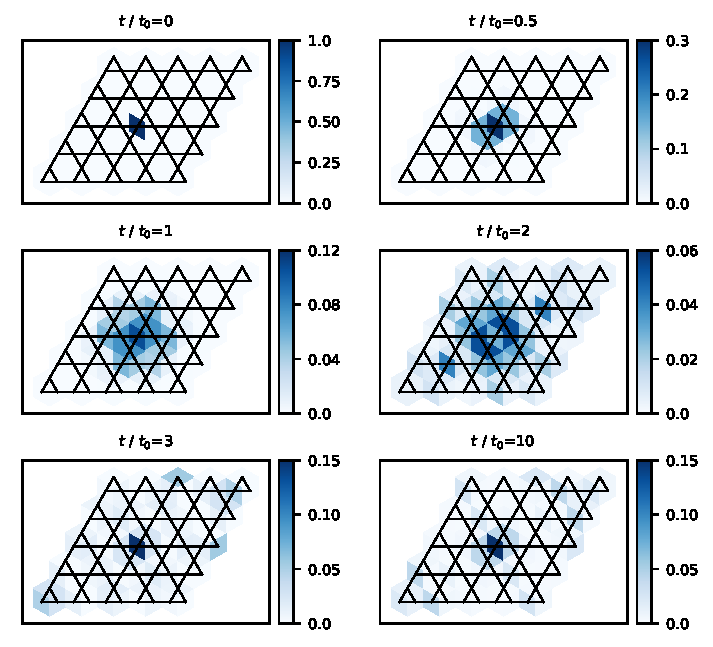
\includegraphics[width=\textwidth]{Figures/Single_Particle_Evolution}
    \caption{Time-evolution of density $\langle n \rangle$ for a single particle initially localised to one site. The small 5$\times$5 unit cell lattice was chosen to enable clear visibility of the expanding density. Note that the colour scale varies between plots. The unit of time is $t_0=\hbar/J$.}
    \label{Fig:Single_Particle_Evolution}
\end{figure}

\section{Stationary Density}\label{Sec:Staionary_Density_1p}

This behaviour can be investigated more quantitatively by calculating the density localised in the vicinity of the original site. This is predicted to tend to $\approx 1/3$, the total density in flat band states. The snapshot of the density in Fig. \ref{Fig:Original_Site_Vicinity_Snapshot} shows that most of the stationary density is localised within the two hexagons containing the original site, corresponding to the flat band hexagon states in Fig. \ref{Fig:Hexagon_Eigenstate}. However, as these states are not a suitable general basis for the flat band, the density in the two hexagons alone is less than 1/3. The most localised orthonormal basis set for the flat band are the Wannier states, which decay $\sim 1/|\textbf{r}|$ from their origin \cite{Huber}. Therefore, to quantify the stationary density, the total density within a small (but arbitrary) radius $r=1.55\,a$ of the original site is plotted in Fig. \ref{Fig:Stationary_Density}. This tends to $0.33 \pm 0.01$, consistent with the theoretical prediction of $1/3$. The fluctuations are due to the dispersive density, which continues to propagate back and forth. This contributes an average density per site of $\approx 2/3$ times the average lattice filling ($1/1200$ for this 20$\times$20 unit cell system), giving a total density of $\approx0.015$ within the $r\leq1.55\,a$ region, consistent with the magnitude of the fluctuations. 

\vspace{1cm}

\begin{figure}[ht]
    \centering
    \sidesubfloat[]{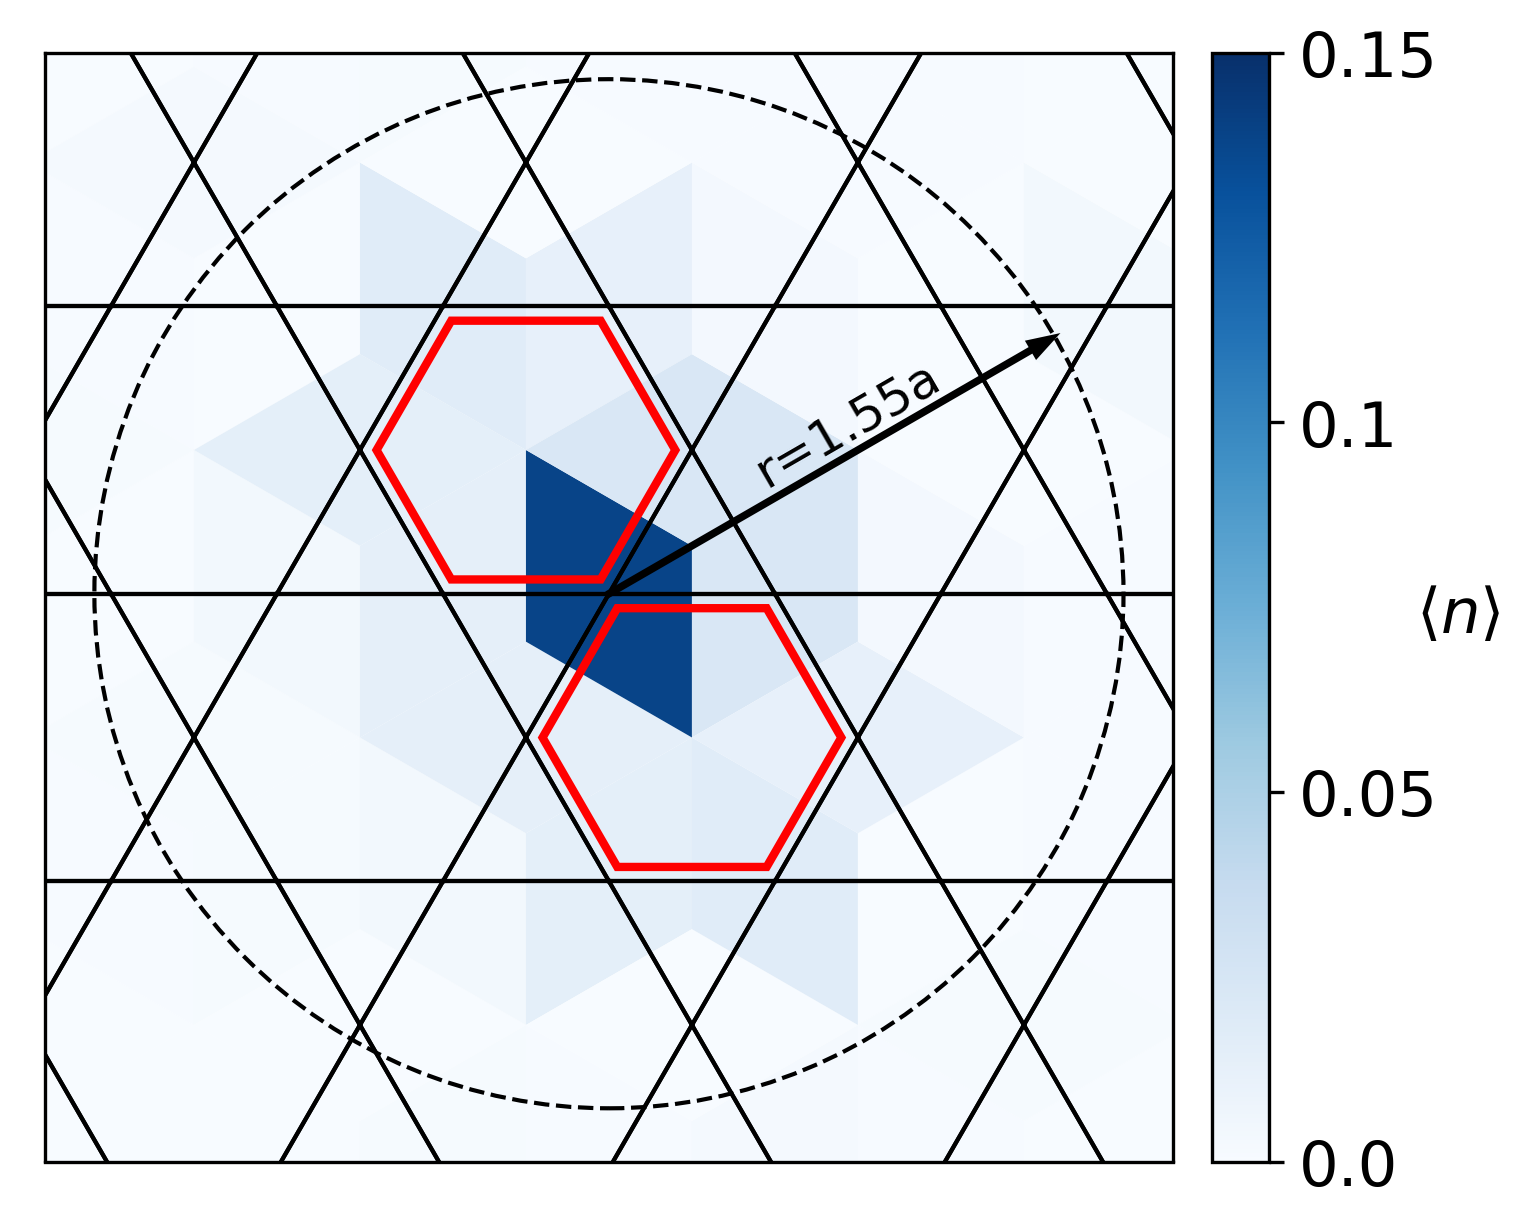
\includegraphics[width=0.46\textwidth]{Figures/Original_Site_Vicinity}\label{Fig:Original_Site_Vicinity_Snapshot}}\hfill
    \sidesubfloat[]{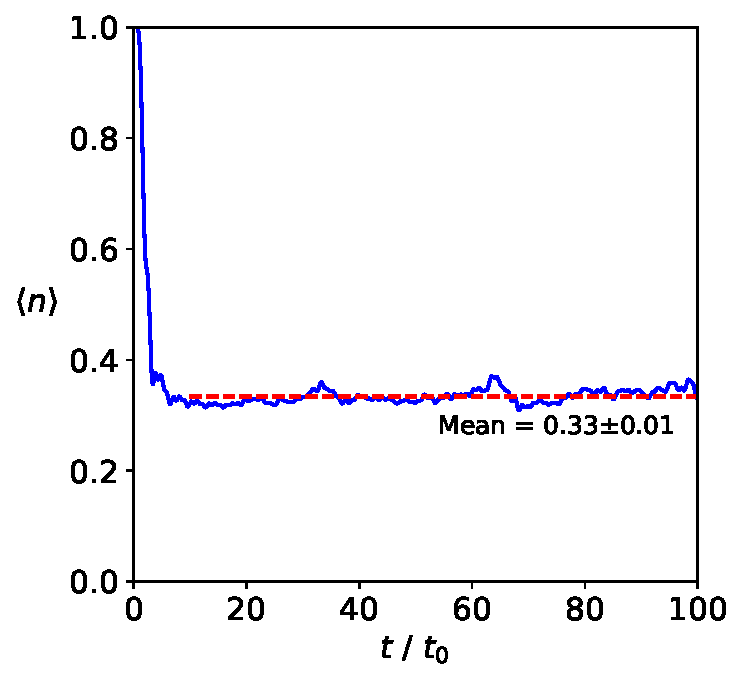
\includegraphics[width=0.45\textwidth]{Figures/Stationary_Density}\label{Fig:Stationary_Density}}
    \caption{Stationary density with a single particle initially localised to one site in a 20$\times$20 unit cell lattice. (a) Snapshot of density at $t=50\,t_0$ in the original site vicinity (the full system extends beyond this region). Most density is contained within the two hexagons indicated in red. (b) Time-evolution of total density (blue, solid) within a radius $r=1.55\,a$ (indicated in (a)) of the original site. The mean (red, dashed) and standard deviation are calculated for $t\geq10\,t_0$. Open boundary conditions were used for this simulation, as the density is susceptible to large fluctuations with periodic boundary conditions.}
    \label{Fig:Original_Site_Vicinity}
\end{figure}